\documentclass[conference]{IEEEtran}

\usepackage[T1]{fontenc}
\usepackage[utf8]{inputenc}
\usepackage{cite}
\usepackage{amsmath,amssymb}
\usepackage{graphicx}
\usepackage{booktabs}
\usepackage{xcolor}
\usepackage{hyperref}
\usepackage{microtype}
\hypersetup{hidelinks}

\begin{document}

\title{Corruption-Agnostic Structural and Generative Ensembling for\\
       Robust Low-Data Digit Recognition}

\author{\IEEEauthorblockN{Attila Torda}
        \IEEEauthorblockA{\textit{Independent Researcher}}}

\maketitle

\begin{abstract}
A strong, reproducible convolutional ensemble (the current MNIST record holder) is also
remarkably data-efficient, reaching $90\%$ test accuracy from only $100$ labelled images.
We ask whether it can be made more robust to image corruptions in the low-data regime by
adding decorrelated, corruption-agnostic members---an interpretable skeleton-graph
classifier and a diffusion-augmented CNN---combined without a held-out split so that every
member trains on the full labelled budget. Against a clean-trained baseline the augmented
ensemble improves mean corruption accuracy at every budget ($+1.7$ to $+4.9$ percentage
points, $8$--$10/10$ seeds). However, an informed baseline that simply augments training
with the test corruptions wins decisively once $\geq\!100$ labels are available, so the
broad gain is illusory in the \emph{known}-corruption setting. We therefore evaluate the
realistic \emph{unknown}-corruption setting via a leave-one-corruption-out protocol: the
augmented baseline is trained on all corruptions \emph{except} the one it is tested on.
There, the corruption-agnostic ensemble generalises to the unseen corruption as well as or
better than targeted augmentation on three of four corruption types (blur, stroke
thickening, occlusion; occlusion by $+7$--$9$~pp at $n\!\geq\!500$); only additive Gaussian
noise resists. The effect reproduces on the harder KMNIST script---where the agnostic ensemble
beats unseen-corruption augmentation on \emph{all four} corruptions at $n\!\geq\!1000$---and
\emph{grows} with corruption severity. The result is a clear, honestly-scoped positive: when the deployment
corruption is unknown, corruption-agnostic structural and generative diversity buys low-data
robustness that targeted augmentation cannot.
\end{abstract}

\begin{IEEEkeywords}
data efficiency, corruption robustness, ensembles, diffusion augmentation, structural
features, MNIST
\end{IEEEkeywords}

\section{Introduction}
Modern convolutional networks reach near-human accuracy on MNIST; the reproducible record is
a majority vote of three ``simple'' CNNs with kernels $3,5,7$ reaching $99.87\%$
\cite{An2020}. Less appreciated is that this ensemble is also strongly data-efficient: in our
re-implementation it reaches $90\%$ test accuracy from $100$ labelled images and $98\%$ from
$500$. This raises a practical question for the small-data regime: such a model is trained on
clean data with geometric augmentation, so how brittle is it to image corruptions it did not
see, and can cheap, decorrelated, \emph{corruption-agnostic} members make it more robust
without additional labels?

We study three members trained on the same small labelled budget: the record holder itself,
an interpretable skeleton-graph bag-of-features classifier whose descriptor is invariant to
stroke thickness by construction, and a CNN trained on images drawn from a small
class-conditional diffusion model. We combine them with held-out-free rules so the baseline
keeps all its labels. Our contributions are: (i) a low-data corruption-robustness benchmark
pairing the MNIST record holder against structural and generative diversity; (ii) an honest
accounting showing that \emph{informed} corruption augmentation is the stronger fix when the
corruption is known and labels are sufficient; and (iii) a leave-one-corruption-out result
showing that, in the realistic unknown-corruption setting, corruption-agnostic diversity
generalises to unseen corruptions as well as or better than targeted augmentation on most
corruption types.

\section{Related Work}
\textbf{MNIST record models.} An et al.\ \cite{An2020} ensemble three deep, pooling-free CNNs
of differing receptive field; we re-implement their architecture (lightly: one model per
kernel, fewer epochs) as the base learner. \textbf{Corruption robustness.} Hendrycks and
Dietterich \cite{Hendrycks2019} standardised common-corruption robustness; MNIST-C
\cite{Mu2019} ports it to digits. We use a compact suite (noise, blur, stroke thickening,
occlusion). \textbf{Structural recognition.} Skeletonisation \cite{GuoHall1989} yields
thickness-invariant descriptors; we classify a $93$-dimensional skeleton-graph vector with a
random forest \cite{Breiman2001}. \textbf{Generative augmentation.} Denoising diffusion models
\cite{Ho2020,Song2021} can synthesise training images; we use a small class-conditional model
as a learned augmenter. \textbf{Ensembles.} Deep ensembles improve robustness and calibration
\cite{Lakshminarayanan2017}; we add \emph{heterogeneous}, decorrelated members rather than
re-seeded copies.

\section{Method}
\subsection{Members}
All members are trained on a class-balanced labelled budget of $n$ clean MNIST images
($n/10$ per digit).
\begin{itemize}
  \item \textbf{Record holder} \cite{An2020}: M3/M5/M7 (kernels $3,5,7$; $10,5,4$ conv layers,
        no pooling, batch-norm, single FC), trained with rotation/translation augmentation;
        combined by majority vote (\texttt{record\_vote}).
  \item \textbf{Structural}: Guo--Hall skeleton \cite{GuoHall1989} $\rightarrow$ $93$-dim
        graph descriptor (endpoints, junctions, loops, orientation/curvature, signed-curvature
        stroke shape) $\rightarrow$ random forest \cite{Breiman2001}.
  \item \textbf{Diffusion} ($n\!\geq\!500$): a small class-conditional DDPM \cite{Ho2020}
        trained on the budget generates a synthetic bank via DDIM \cite{Song2021}; a CNN is
        trained on the budget plus the bank.
\end{itemize}

\subsection{Held-out-free combiners}
To avoid starving the baseline of labels, combiners use no held-out split: \texttt{soft}
(equal mean of member probabilities) and \texttt{conf} (per-sample confidence-weighted mean,
weight $\propto$ each member's max-probability on the image). Both let all members---including
the record holder's CNNs---train on the full budget.

\subsection{Corruptions and protocol}
We evaluate on the $10$k test set under \texttt{clean}, \texttt{gaussian\_noise},
\texttt{blur}, \texttt{stroke\_dilate}, and \texttt{occlusion} (one moderate severity each).
Members are trained on \emph{clean} data; corruption affects test images only. We report
per-corruption accuracy and mean corruption accuracy (mCA) over the four non-clean
corruptions, averaged over $10$ seeds. We compare against two baselines: \texttt{record\_vote}
(clean-trained) and \texttt{record\_aug} (the record holder retrained with the corruptions
mixed into its augmentation---the ``if you know the corruption, train for it'' baseline).

\subsection{Leave-one-corruption-out (LOCO)}
\texttt{record\_aug} is unrealistically advantaged: it trains on the exact corruption it is
tested on. We therefore train it on all corruptions \emph{except} the held-out one
(\texttt{record\_aug\_loco}) and test on the held-out (unseen) corruption, the deployment-%
realistic setting in which the corruption is unknown at training time. The
corruption-agnostic ensemble is unchanged across held-out corruptions.

\section{Results}
\subsection{Robustness over the clean-trained baseline}
Table~\ref{tab:mca} reports mCA. The augmented ensemble (\texttt{conf\_all}) beats the
clean-trained record holder at every budget ($+1.7$ to $+4.9$~pp; $8$--$10/10$ seeds improve).
Figure~\ref{fig:mca} shows the curves. A leave-one-member-out ablation
(Fig.~\ref{fig:attr}) attributes the gain by regime: the \emph{structural} member drives the
low-budget gain (e.g.\ $+3.3$~pp on \texttt{stroke\_dilate} at $n\!=\!100$, consistent with
thickness invariance), while the \emph{diffusion} member drives the $n\!\geq\!500$ gain
($+3.2$ to $+4.7$~pp), concentrated on \texttt{gaussian\_noise} and \texttt{occlusion}.

\begin{table}[t]
\caption{Mean corruption accuracy (mCA, \%), $10$ seeds.}
\label{tab:mca}
\centering
\begin{tabular}{@{}lccc@{}}
\toprule
$n$ & \texttt{record\_vote} & \texttt{conf\_all} & \texttt{record\_aug} \\
\midrule
20   & 49.8 & \textbf{51.5} & 42.7 \\
50   & 62.4 & 63.6 & 63.8 \\
100  & 67.7 & 69.0 & \textbf{75.8} \\
200  & 68.1 & 68.6 & \textbf{84.1} \\
500  & 66.9 & 70.6 & \textbf{90.1} \\
1000 & 67.8 & 72.1 & --- \\
2000 & 68.6 & 73.5 & --- \\
\bottomrule
\end{tabular}
\end{table}

\subsection{The honest limit: informed augmentation wins}
The \texttt{record\_aug} column of Table~\ref{tab:mca} is decisive: once $\geq\!100$ labels are
available, simply training on the corruptions beats the agnostic ensemble by $+6.8$ to
$+19.4$~pp. The agnostic ensemble out-performs it at only one budget, $n\!=\!20$ ($+8.8$~pp,
$10/10$ seeds), where so few labels make it impossible to learn classification \emph{and}
corruption invariance in a single network. Thus in the known-corruption setting there is no
broad win.

\subsection{The realistic setting: unseen corruptions (LOCO)}
Table~\ref{tab:loco} reports \texttt{conf\_all}~$-$~\texttt{record\_aug\_loco} on the
held-out (unseen) corruption (Fig.~\ref{fig:loco}). On three of four corruptions---blur,
stroke thickening, and occlusion---the corruption-agnostic ensemble matches or beats targeted
augmentation that never saw the corruption, strongly so for occlusion ($+7$ to $+9$~pp at
$n\!\geq\!500$). Only \texttt{gaussian\_noise} resists: it must be seen to be handled.

\begin{table}[t]
\caption{LOCO: \texttt{conf\_all} $-$ \texttt{record\_aug\_loco} on the \emph{unseen}
         corruption (pp). Positive favours the agnostic ensemble.}
\label{tab:loco}
\centering
\begin{tabular}{@{}lrrrrr@{}}
\toprule
held-out & $100$ & $200$ & $500$ & $1000$ & $2000$ \\
\midrule
blur            & $+4.6$ & $+2.2$ & $-0.4$ & $+1.5$ & $+1.0$ \\
stroke\_dilate  & $+7.3$ & $+1.1$ & $-2.9$ & $+0.5$ & $+0.4$ \\
occlusion       & $+2.1$ & $+0.9$ & $+7.4$ & $+8.7$ & $+8.0$ \\
gaussian\_noise & $-2.1$ & $-14.4$& $-1.0$ & $-3.9$ & $+2.0$ \\
\bottomrule
\end{tabular}
\end{table}

\subsection{Generality to a harder script (KMNIST)}
Repeating the study on KMNIST \cite{Clanuwat2018}, a harder $10$-class cursive-Japanese set,
reproduces the pattern. The agnostic ensemble improves mCA once the diffusion member is active
($+3.8$~pp at $n\!=\!1000$, $+3.4$ at $n\!=\!2000$; $10/10$ seeds), and informed augmentation
again wins at intermediate budgets. Under the leave-one-corruption-out protocol
(Table~\ref{tab:kmnistloco}, Fig.~\ref{fig:kmnistloco}) the agnostic ensemble beats
unseen-corruption augmentation on \emph{all four} corruptions at $n\!\geq\!1000$---including
gaussian noise, which had resisted on MNIST---so the effect is not specific to MNIST.

\begin{table}[t]
\caption{KMNIST LOCO: \texttt{conf\_all} $-$ \texttt{record\_aug\_loco} on the \emph{unseen}
         corruption (pp). Positive favours the agnostic ensemble.}
\label{tab:kmnistloco}
\centering
\begin{tabular}{@{}lrrrrr@{}}
\toprule
held-out & $100$ & $200$ & $500$ & $1000$ & $2000$ \\
\midrule
blur            & $+2.1$ & $+2.8$ & $+2.0$ & $+2.0$ & $+4.0$ \\
stroke\_dilate  & $+5.9$ & $+1.4$ & $-2.1$ & $+1.0$ & $+0.5$ \\
occlusion       & $+5.1$ & $+3.7$ & $+2.4$ & $+3.7$ & $+4.1$ \\
gaussian\_noise & $-1.2$ & $-3.8$ & $+6.5$ & $+8.8$ & $+4.3$ \\
\bottomrule
\end{tabular}
\end{table}

\subsection{Severity dependence}
Figure~\ref{fig:sev} sweeps corruption severity at $n\!=\!2000$. The advantage is not an
artefact of a single severity: it \emph{grows} with severity, peaking where the record holder
degrades most---blur $+20$~pp at $\sigma\!=\!2.0$, occlusion $+16$~pp at side $14$, stroke
$+10$~pp at radius $3$---and only vanishes under near-destructive Gaussian noise, where every
method approaches chance.

\begin{figure}[t]
\centering
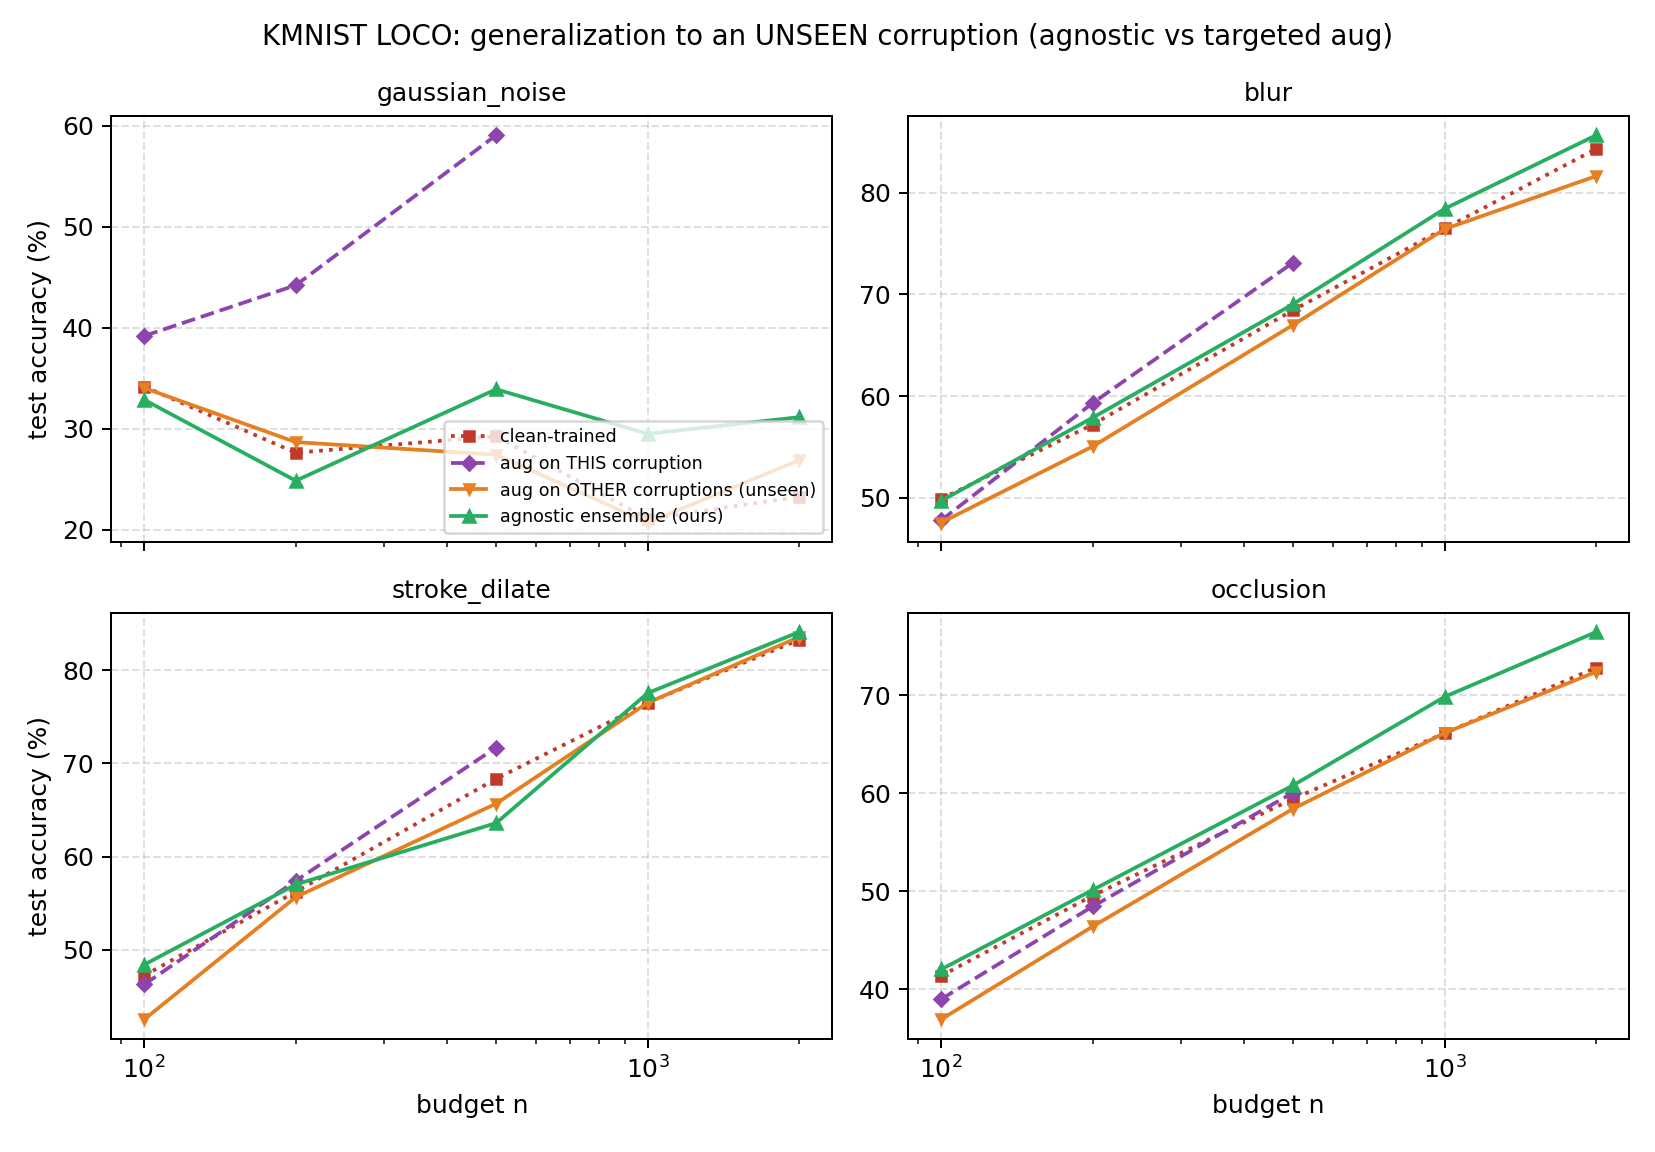
\includegraphics[width=\columnwidth]{figures/fig13_track9c_kmnist_loco.png}
\caption{KMNIST leave-one-corruption-out. The corruption-agnostic ensemble (green) matches or
beats augmentation trained on the \emph{other} corruptions (orange) at the unseen corruption on
all four types for $n\!\geq\!1000$.}
\label{fig:kmnistloco}
\end{figure}

\begin{figure}[t]
\centering
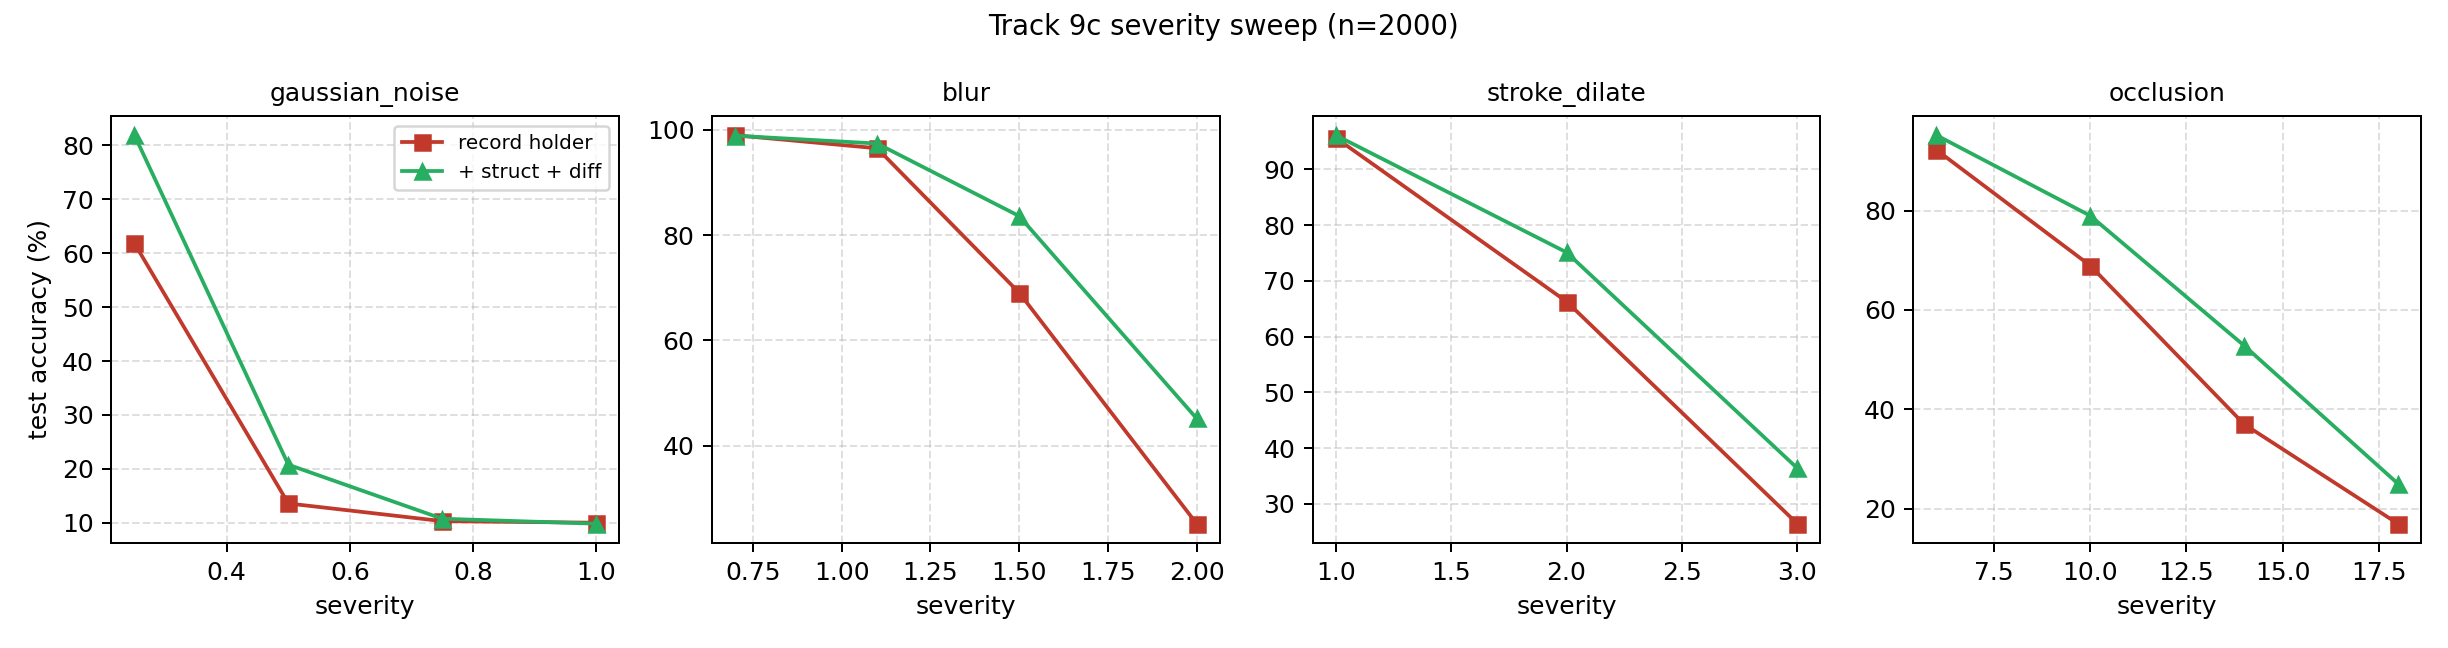
\includegraphics[width=\columnwidth]{figures/fig12_track9c_severity.png}
\caption{Severity sweep at $n\!=\!2000$. The agnostic ensemble's advantage over the record
holder grows with corruption severity, except under near-destructive Gaussian noise.}
\label{fig:sev}
\end{figure}

\begin{figure}[t]
\centering
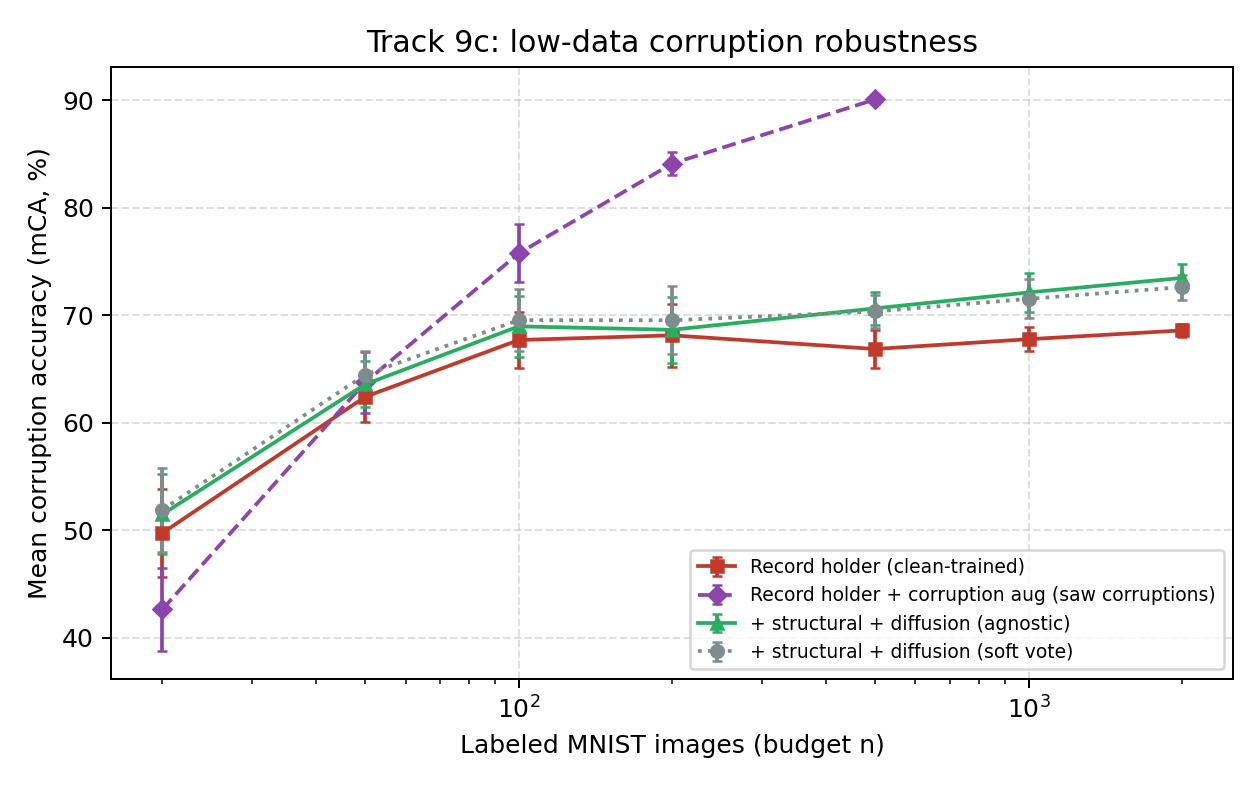
\includegraphics[width=\columnwidth]{figures/fig9_track9c_mca.png}
\caption{Mean corruption accuracy versus labelled budget. The agnostic ensemble
(\texttt{conf\_all}) beats the clean-trained record holder everywhere; informed augmentation
(\texttt{record\_aug}, dashed) is stronger once $\geq\!100$ labels are available.}
\label{fig:mca}
\end{figure}

\begin{figure}[t]
\centering
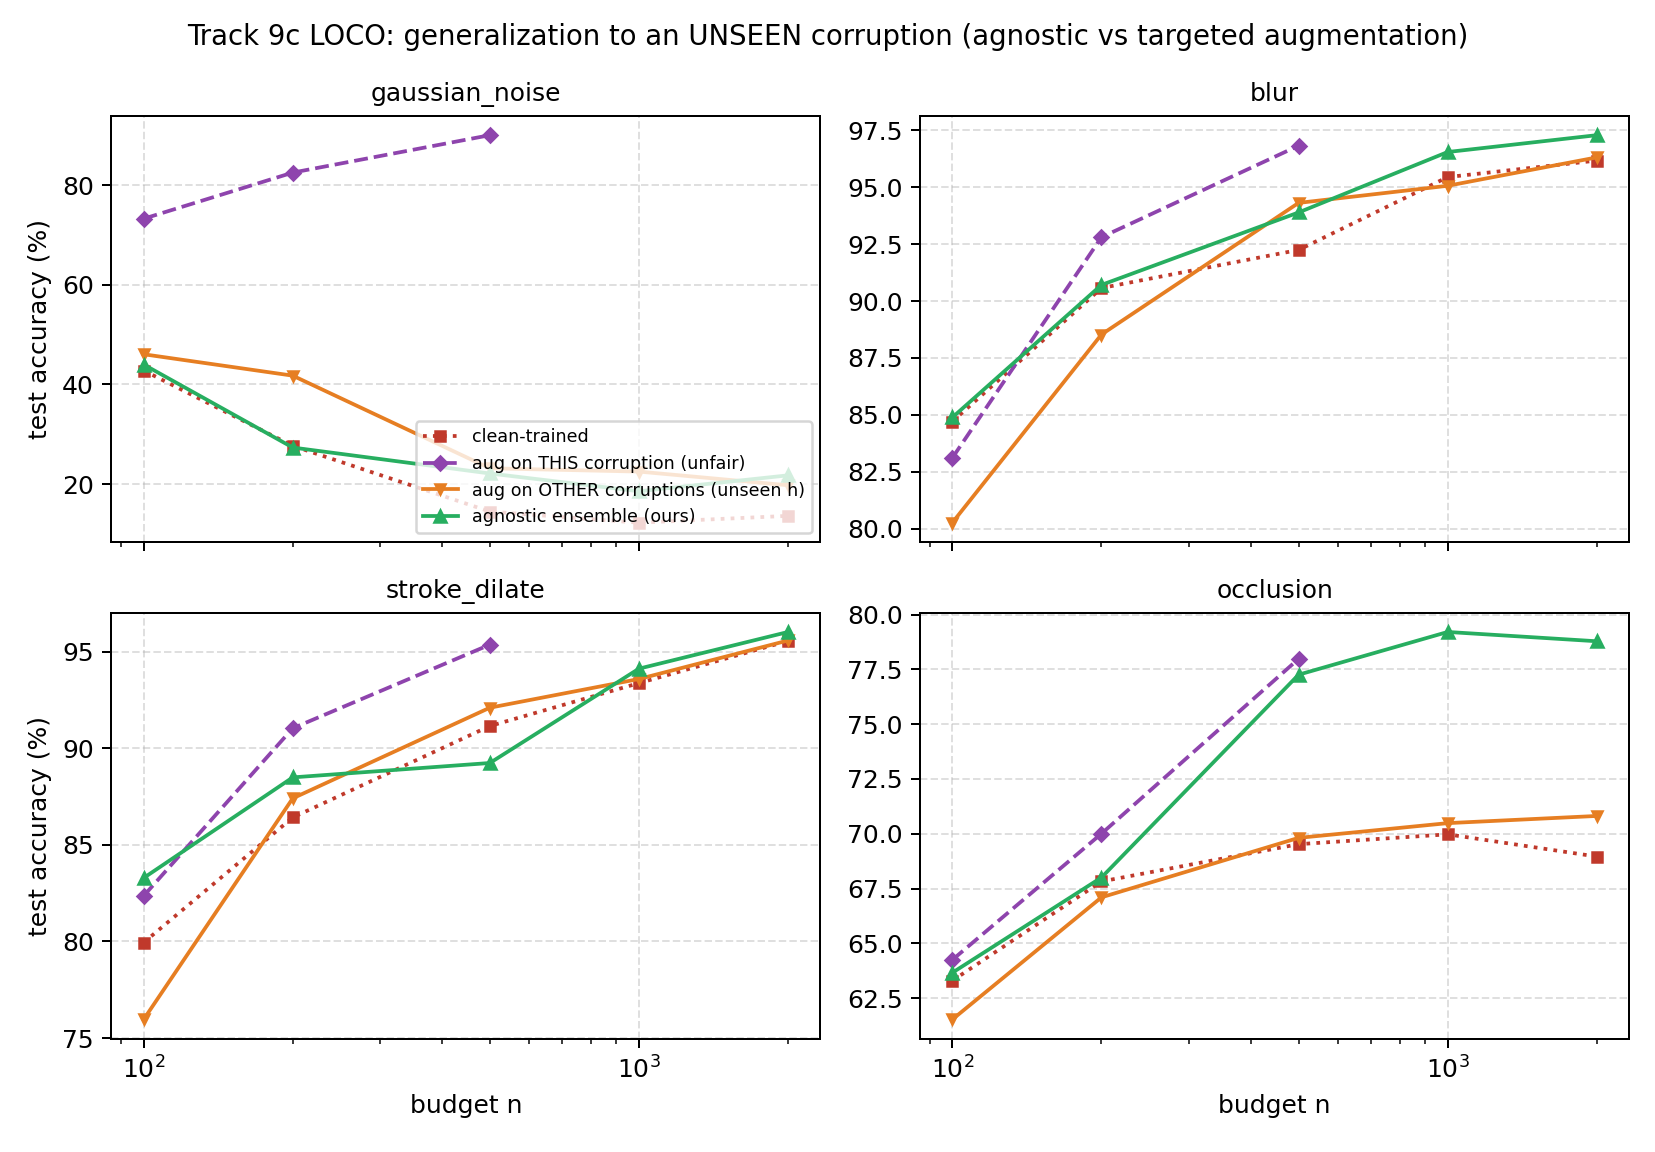
\includegraphics[width=\columnwidth]{figures/fig10_track9c_loco.png}
\caption{Leave-one-corruption-out. On blur, stroke thickening and occlusion the
corruption-agnostic ensemble (green) matches or beats augmentation trained on the other
corruptions (orange) at the unseen corruption; gaussian noise is the exception.}
\label{fig:loco}
\end{figure}

\begin{figure}[t]
\centering
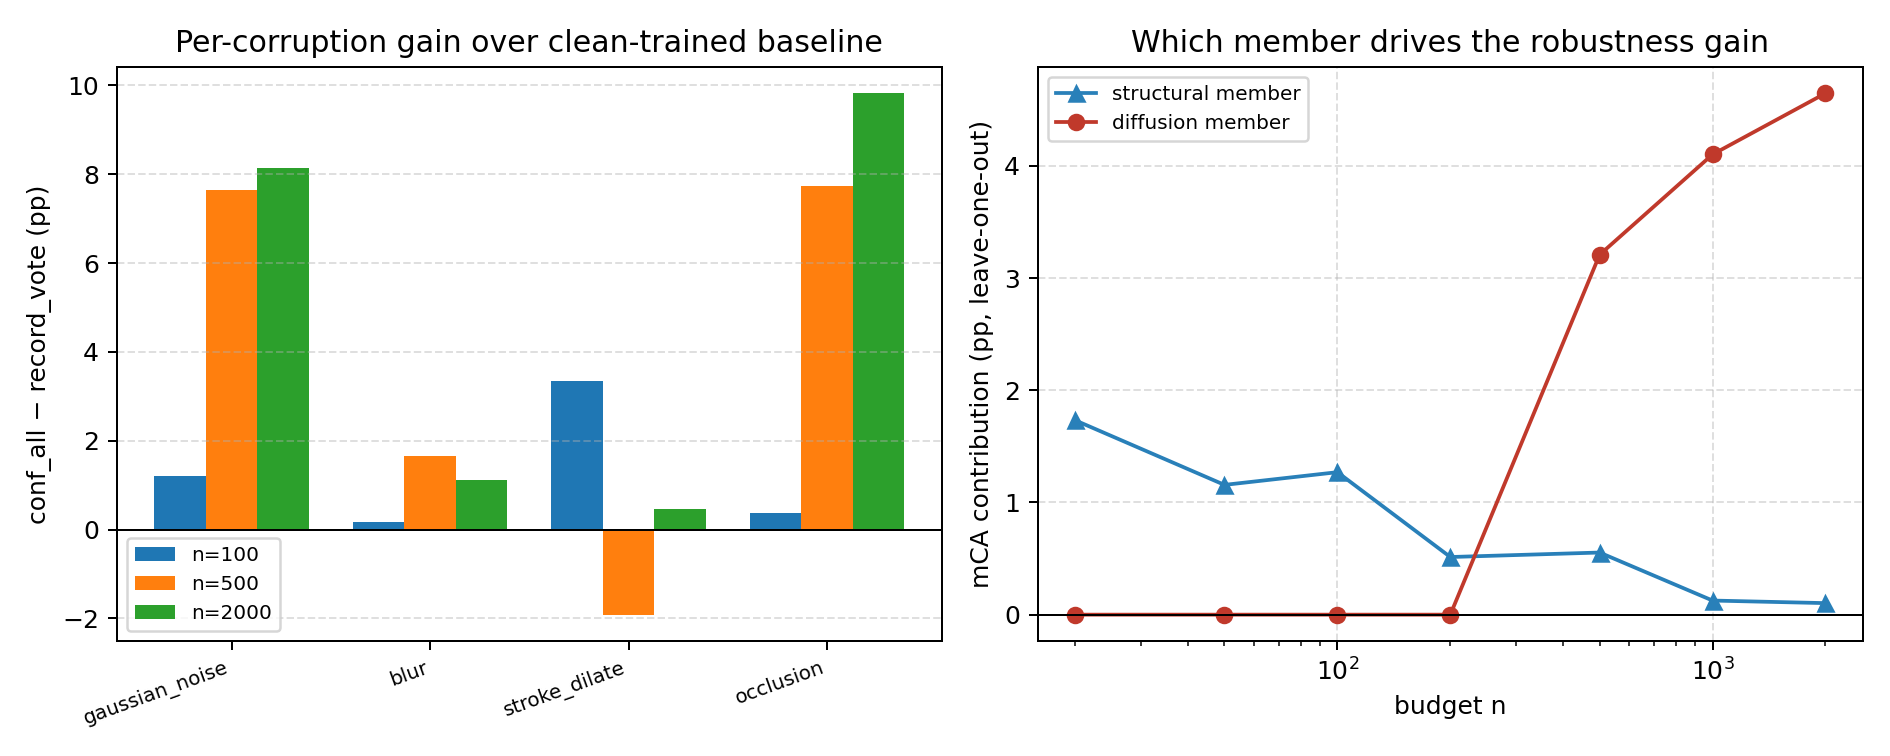
\includegraphics[width=\columnwidth]{figures/fig11_track9c_attribution.png}
\caption{Left: per-corruption gain of \texttt{conf\_all} over the clean-trained baseline.
Right: leave-one-member-out mCA contribution---structural at low $n$, diffusion at
$n\!\geq\!500$.}
\label{fig:attr}
\end{figure}

\section{Discussion and Limitations}
The positive is real but narrowly scoped, and we state the boundaries plainly.
(i)~\textbf{Threat model.} The win is in the \emph{unknown}-corruption setting; if the
corruption is known and $\geq\!100$ labels exist, targeted augmentation is far stronger.
(ii)~\textbf{Gaussian noise} defeats the approach---skeletonisation is noise-fragile and
clean-trained CNNs are noise-fragile---so the agnostic ensemble cannot generalise to it
unseen. (iii)~\textbf{The combiner is not the hero}: confidence weighting (\texttt{conf}) is
no better than plain averaging (\texttt{soft}); the gain comes from member diversity, not the
combination rule. (iv)~\textbf{Mechanism is mixed}: stroke-thickness invariance only carries
the low-budget stroke gain; the larger gains are from the diffusion (generative-augmentation)
member. (v)~The gain needs the diffusion member and hence $\geq\!500$ labels; below that only
the structural member contributes and the effect is small. The corruption suite, though now
swept over severity and reproduced on a second script (KMNIST), remains synthetic---physical
corruptions are untested.

\section{Conclusion}
A reproducible MNIST record ensemble is highly data-efficient but brittle to unseen
corruptions in the low-data regime. Adding corruption-agnostic structural and generative
members---combined without sacrificing labels to a held-out split---improves its robustness
to corruptions it was not trained for, generalising to unseen blur, stroke thickening and
occlusion as well as or better than targeted augmentation. The effect reproduces on the harder
KMNIST script and grows with corruption severity. When the deployment corruption is unknown,
corruption-agnostic diversity is a label-free robustness lever; when it is known, train for it.

\section*{Reproducibility}
Experiments: \texttt{scripts/run\_track9\_robust.py} (mCA, ablation),
\texttt{scripts/run\_track9\_loco.py} (LOCO). Models and corruptions:
\texttt{src/track9/}. Raw results: \texttt{track9\_robust\_results.json},
\texttt{track9\_loco\_results.json}.

\bibliographystyle{IEEEtran}
\bibliography{track9c_refs}

\end{document}
